%==============================================================================
% Importando a classe
%==============================================================================
\documentclass{templufla}          


%==============================================================================
% Configuração dos pacotes necessários
%==============================================================================
% Primeiros pacotes (alguns precisam ser importados depois)

% TEXTOS
\usepackage[brazil]{babel}       % hifenização e títulos em português do Brasil
\usepackage[T1]{fontenc}         % usa fontes postscript com acentos
\usepackage[utf8]{inputenc}      % permite edição direta com acentos
\usepackage{listings}            % para inserção de código
\usepackage{fancyvrb}            % para inserção de saídas de comandos

% MATEMÁTICA
\usepackage{amsmath}             % pacote da AMS para Matemática Avançada
\usepackage{amssymb}             % símbolos extras da AMS
\usepackage{mathtools}			 % para mais comandos de matemática
\usepackage{latexsym}            % símbolos extras do LaTeX

% TABELAS
\usepackage{longtable}           % para tabelas muito grandes
\usepackage{array}               % para mais opções em tabelas
\usepackage{colortbl}            % para cores em tabelas
\usepackage{multirow}            % para células com várias linhas
\usepackage{multicol}            % para células com várias colunas

% FIGUAS E GRÁFICOS
\usepackage{xcolor}              % para mais cores
\usepackage{subfigure}           % para figuras dentro de figuras
\usepackage{caption}             % para remodelar o formato dos títulos

%==============================================================================
% O pacote hyperref para referência cruzadas dentro do documento \ref e \autoref

% Setspace precisa estar antes do hyperref para usar a versão atual do abntex.
\usepackage{setspace}

% Definindo cores para os links cruzados
\definecolor{rltred}{rgb}{0.2,0,0}
\definecolor{rltgreen}{rgb}{0,0.2,0}
\definecolor{rltblue}{rgb}{0,0,0.2}


% Importa hyperref
\usepackage[%
hidelinks, % colorlinks=true, | Troque se quiser link com cor
urlcolor=rltblue,       % \href{...}{...} external (URL)
filecolor=rltgreen,     % \href{...} local file
linkcolor=rltred,       % \ref{...} and \pageref{...}
citecolor=rltgreen,%
]{hyperref} % 


%==============================================================================
% Citações/referências no formato ABNT, utilizando o pacote abntex2.
% O pacote já vem na maioria das distribuições (texLive, MikTeX, Overleaf e etc...)
% mas, caso você seja super roots e não use os listados, precisa instalar o abntex2:
% http://abntex.codigolivre.org.br/

% A versão disponível com esse template sofreu algumas alterações para se adaptar ao
% padrão atual, já que a original está desatualizada.
% Para mais informações, vizite o repositório oficial do template.


% abnt-emphasize=bf coloca o título das bibliografias em negrito
% abnt-etal-list=3 limita o número de autores antes de et al. para 3
% abnt-url-package=xurl diz para usar o pacote xurl
\usepackage[alf, abnt-etal-list=3, abnt-url-package=xurl, abnt-emphasize=bf]{abntex2cite}

%==============================================================================
% Ajustando os pacotes importados

% Definindo cores para elementos tabulares
\newcolumntype{Z}{|>{\columncolor[gray]{0.9}}l|} %cor cinza em células
\newcolumntype{L}[1]{>{\raggedright\let\newline\\\arraybackslash\hspace{0pt}}m{#1}}
\newcolumntype{C}[1]{>{\centering\let\newline\\\arraybackslash\hspace{0pt}}m{#1}}
\newcolumntype{R}[1]{>{\raggedleft\let\newline\\\arraybackslash\hspace{0pt}}m{#1}}

% Definindo espaçamento vertical de elementos tabulares
\renewcommand{\arraystretch}{1.5}

% Configuração padrão do listings (ambiente de código)
\lstset{
	extendedchars=true,
	breaklines=true,
	tabsize=3,
	basicstyle=\linespread{1}\ttfamily\normalsize,
	stringstyle=\em,
	showstringspaces=true,
	inputencoding=utf8,
	captionpos=t,
	backgroundcolor=\color{black!5},
	literate={{á}{{\'a}}1 {é}{{\'e}}1 {í}{{\'i}}1 {ó}{{\'o}}1 {ú}{{\'u}}1
	{Á}{{\'A}}1 {É}{{\'E}}1 {Í}{{\'I}}1 {Ó}{{\'O}}1 {Ú}{{\'U}}1
	{â}{{\^a}}1 {ê}{{\^e}}1 {ô}{{\^o}}1
	{Â}{{\^A}}1 {Ê}{{\^E}}1 {Ô}{{\^O}}1
	{ã}{{\~a}}1 {õ}{{\~o}}1 {ẽ}{{\~e}}1 
	{ç}{{\c{c}}}1
	{à}{{\`{a}}}1{À}{{\`{A}}}1}
}

% Carregamento do glossário, listas de siglas, símbolos e etc
\loadglsentries{glossarios/abreviaturas}
\loadglsentries{glossarios/glossario}
\loadglsentries{glossarios/siglas}
\loadglsentries{glossarios/simbolos}

% Especificando hifenizações que por ventura LaTeX não saiba fazer
% Por padrão 99,9% dos termos em português devem ser hifenizados corretamente.
% Adicione aqui palavras precise especificar como hifenizar (ou não hifenizar)
\hyphenation{software am-bien-te coor-de-na-ção FAE-PE TelEduc Williams UFLA Murray Bookchin}

% Adaptando os nomes das seções
% Também pode ser usado para alterar a lingua dos elementos
% (ex Figura para Figure, caso seu texto esteja em inglês).
\addto\captionsbrazil{
	\renewcommand{\chaptername}{Seção}
	\renewcommand{\subsectionname}{Seção}
	\renewcommand{\subsubsectionname}{Seção}
	%\renewcommand{\figurename}{Figure}
}
\addto\extrasbrazil{
	\renewcommand{\chapterautorefname}{Seção}
	\renewcommand{\subsectionautorefname}{Seção}
	\renewcommand{\subsubsectionautorefname}{Seção}
	%\renewcommand{\figureautorefname}{Figure}
}


%==============================================================================
% Dados da monografia, capa: autor, titulo, banca, etc... - SUBSTITUA DE ACORDO
%==============================================================================
% Dados para o arquivo PDF (metadados)
\hypersetup{%
% Titulo
pdftitle={Template de Exemplo do Estilo Padrão UFLA},
% Autor
pdfauthor={Joana Autora da Silva},
% Descrição
pdfsubject={Um template de trabalhos acadêmcios UFLA em LaTeX, atualizado com a 6ª edição.},
% Palavras-Chave
pdfkeywords={comunicação científica; pesquisa; pesquisa científica; redação.}
}
	
%==============================================================================
% Informações básicas

% Nome da(s)/do(s) autora(s)/autor(es)
\author{Joana Autora da Silva}

% Título do trabalho, em lígua vernácula
\title{Template de Exemplo do Estilo Padrão UFLA}

% Subítulo do trabalho, em lígua vernácula
\subtitle{Usando Latex! =)}

% Título do trabalho, em inglês
\engtitle{Example Template for UFLAS' Standard Style}

% Subítulo do trabalho, em inglês
\engsubtitle{Using \LaTeX =)}

% Edição, se houver. Caso contrário, comente.
\edicao{6$^a$ edição atualizada, ampliada e revista}

% Data de publicação
\date{2025}

% Tipo do Documento
\tipo{Tese apresentada à Universidade Federal de Lavras, como parte das exigências do Programa de Pós-Graduação em Monografia, área de concentração em TCC, para a obtenção do título de Doutor. }


% Orientador/orientadora
% Altere o comando para os diferentes gêneros
\orientador{Prof. DSc. José Orientador}
%\orientadora{Profa. DSc. Maria Orientadora}

% Coorientador/coorientadora
% Altere o comando para os diferentes gêneros
% Comente se não houver.
\coorientadora{Profa. DSc. Maria Orientadora }
%\coorientador{Prof. DSc. José Orientador}

% Local
\local{Lavras -- MG}

%==============================================================================
% Informações da banca

% Membros da banca. Até quatro membros. 
% Deve ser {nome}{instituição}.
% Comente os últimos se a banca tiver menos membros.
\bancaum{Prof. MSc. Antônio Banca Um}{UFM}
\bancadois{Prof. DSc. João Banca Dois}{FCO}
\bancatres{Profa. Esp. Eliza Banca Três}{BELMIS}
\bancaquatro{Prof. Esp. Zorbison Uberplax IV}{UFO}

% Data da defesa
\defesa{29 de maio de 2025}

%==============================================================================
% Dados para Ficha catalográfica, gerada pelo sistema da Biblioteca da UFLA
% http://www.biblioteca.ufla.br/FichaCatalografica/
% dados para ficha catalográfica

% Texto acima da ficha
\preparofichacat{Ficha catalográfica elaborada pela Coordenadoria de Processos Técnicos da Biblioteca Universitária da UFLA, com dados informados pelo(a) próprio(a) autor(a).}

% Primeiro autor - como na primeira linha da ficha catalográfica
\fcautor{Silva, Joana Autora da}

% Autores, separados por vírgula - na ficha catalográfica, no formato que
% vem após o título e a barra ("/")
\fcautores{Joana Autora da Silva, João Autor do Silvo}

% Numero de páginas,
% Caso o valor seja diferente do calculado, basta descomentar e adicionar.
%\fcnpaginas{777}

% Caso trabalho seja ilustrado (figuras, gráficos, tabelas, etc.).
% Caso não seja ilustrado, basta comentá-lo
\fcilustrado{il.}

% Dados da edição para a ficha 
\fcedicao{6$^a$ ed. rev., atual. e ampl.}

% Tipo do trabalho (tese, dissertação, etc.), de acordo com sistema
% de geração de ficha catalográfica
\fctipo{Tese(doutorado)}

% Ano da defesa, só precisa informar se for diferente do ano da publicação
% se forem iguais, comente a linha a seguir
%\fcdatadefesa{2025}

% Preencher aqui com os dados de catalogação gerados pelo sistema
\fccatalogacao{1. TCC. 2. Monografia. 3. Dissertação. 4. Tese. 5. Trabalho Científico – Normas. I. Universidade Federal de Lavras. II. Título.}
\fcclasi{808.066}

%==============================================================================
% Se vc já defendeu e tem o arquivo escaneado da folha de rosto, 
% descomente e altere o nome do arquivo
%\folhaAprovacaoAssinada{folharosto}


%==============================================================================
% O documento em si
%==============================================================================
\begin{document}

%==============================================================================
%Elementos pré-textuais

% Cria capa, folha de rosto, folha de aprovação e ficha
\maketitle

% Dedicatórias\\
\dedic{Espaço reservado à dedicatória.}

% Agradecimentos
\thanks{Espaço reservado aos agradecimentos.}         

% Epígrafe
\epigrafe{%
Espaço reservado à epígrafe.\par
(Autor Desconhecido)}

% Resumo e palavras-chave
% As palavras-chave PRECISAM vir primeiro
\palchaves{resumo; palavras; representativas.}
\resumo{%
O resumo deve conter palavras representativas do conteúdo do trabalho, localizadas abaixo do mesmo, antecedidas da expressão “palavras-chave” seguida de dois pontos. As palavras-chave devem ser separadas entre si por ponto e vírgula e finalizadas por ponto. Devem ser grafadas com as iniciais em letra minúscula, com exceção dos substantivos próprios e nomes científicos.
}

% Abstract e keywords
% As keywords PRECISAM vir primeiro
\keywords{summary; words; representative.}
\abstract{%
The abstract must contain words representative of the content of the work, located below it, preceded by the expression “keywords” followed by two points. Keywords should be separated from each other by semicolons and finalized by periods. They should be spelled with the initials in lowercase, with the exception of proper nouns and scientific names.
}

% Indicadores de impacto
\indicadoresdeimpacto{%
De caráter institucional, é um item obrigatório como parte das exigências das PRPG/PROEC para os trabalhos de pós-graduação Stricto sensu da UFLA. O autor deve apresentar um relato dos impactos sociais, tecnológicos, econômicos e/ou culturais dos resultados obtidos, considerando as populações, sociedade e territórios, deixando evidente se esses impactos foram concretos e diretos ou em potencial. Ao elaborar o item sobre impactos, é importante: 
a) caracterizar e quantificar resultados dos impactos sociais, tecnológicos, econômicos e/ou culturais da melhor forma possível; 
b) estabelecer se há algum caráter extensionista no trabalho, demonstrando impacto e participação da sociedade externa à UFLA, como parceiros e público-alvo; 
c) definir o território e grupos populacionais impactados; 
d) quando possível, declarar público diretamente beneficiado e número de docentes, estudantes e técnicos envolvidos nas ações extensionistas; 
e) estabelecer em quais das oito áreas temáticas da Política Nacional de Extensão podem ser classificados os impactos do trabalho. São elas: 1 - Comunicação, 2 - Cultura, 3 - Direitos humanos e justiça, 4 - Educação, 5 - Meio ambiente, 6 - Saúde, 7 - Tecnologia e produção e 8 - Trabalho;
f) demonstrar quais os impactos da pesquisa e se estão alinhados com os 17 (dezessete) Objetivos de Desenvolvimento Sustentável (ODS) da Organização das Nações Unidas (ONU).
}

% Impact indicators
\impactindicators{%
Of an institutional nature, it is a mandatory item as part of the PRPG/PROEC requirements for UFLA's Stricto sensu postgraduate work. The author must present a report on the social, technological, economic and/or cultural impacts of the results obtained, considering the populations, society and territories, making it clear whether these impacts were concrete and direct or potential. When preparing the item on impacts, it is important to:
a) characterize and quantify the results of the social, technological, economic and/or cultural impacts in the best possible way;
b) establish whether there is any extensionist character to the work, demonstrating the impact and participation of society outside UFLA, such as partners and target audience;
c) define the territory and population groups impacted;
d) when possible, declare the public directly benefited and the number of teachers, students and technicians involved in the extension actions;
e) establish in which of the eight thematic areas of the National Extension Policy the impacts of the work can be classified. They are: 1 - Communication, 2 - Culture, 3 - Human rights and justice, 4 - Education, 5 - Environment, 6 - Health, 7 - Technology and production and 8 - Work;
f) demonstrate the impacts of the research and whether they are aligned with the 17 (seventeen) Sustainable Development Goals (SDGs) of the United Nations (UN).
}

% Listas gerais
% Comente para remover.
\listoffigures  	% Lista de Figuras
%\listofilustracoes % Lista de Ilustrações
%\listofgraficos	% Lista de Gráficos
\listoftables       % Lista de Tabelas
\listofquadros		% Lista de Quadros
%\listofexemplos    % Lista de Exemplos
%\listofteoremas    % Lista de Teoremas
\listofabreviaturas % Lista de Abreviaturas
\listofsiglas       % Lista de Siglas
\listofsimbolos     % Lista de Símbolos

% Sumário
\tableofcontents
\clearpage

%==============================================================================
% Elementos textuais

% Começa a mostrar a numeração
\pagestyle{ufla}


% Incluindo as seções
% É recomendado que as seções sejam organizadas em arquivos separados
% e incluídas no documento com o comando \include
\chapter{\MakeUppercase{Introdução}}

O objetivo deste documento é apresentar o uso básico da classe \texttt{templufla} para a elaboração de trabalhos acadêmicos da \glsxtrfull{ufla}, utilizando a linguagem de marcação \LaTeX\ \cite[ p.17]{Lamport1994}. A maioria dos comandos (macros) e ambientes das classes básicas da linguagem é válida também nessa classe, que é estendida com comandos para confecção da capa, páginas de rosto, dedicatórias, etc. A classe atual foi baseada na classe \texttt{uflamon}, disponível em CC-BY 4.0, no site Overleaf.

Inicialmente, a classe \texttt{uflamon} foi criada de acordo com as normas da PRPG/UFLA para produção de TCC \cite{PRPG2006}. Essas normas foram posteriormente atualizadas, de maneira geral pela UFLA, para a produção de monografias, dissertações e teses \cite{BIB2010}. A classe \texttt{uflamon} foi mantida até a 2ª edição da normalização da \gls{ufla} \cite{UFLA:2015}.

Então, em 2025, com a publicação da 6ª edição da normalização \cite{UFLA:2025}, os atuais mantenedores criaram a classe \texttt{templufla} e o atual template, adaptando o antigo código para a nova norma, corrigindo inadequações, atualizando pacotes e ampliando o formato.

Este texto, com o objetivo de familiarizar o usuário da linguagem \LaTeX\ e demonstrar o uso da classe \texttt{templufla}, encontra-se organizado da seguinte maneira: 

A \autoref{sec:latex} apresenta conceitos básicos da linguagem \LaTeX, servindo como um ponto de início para novos usuários. 
A \autoref{sec:template} demonstra como utilizar os elementos da classe para a criação de trabalhos no formato da \gls{ufla}.
A \autoref{sec:listasEGlossario} é um tutorial básico de como usar os pacotes \texttt{glossaries} e \texttt{imakeidx} para criar listas, glossário e índice. 
A \autoref{sec:conclusao} apresenta comentários e observações finais.
Por fim, os Anexos \ref{anex:lorem1} e \ref{anex:lorem2} demonstram o uso dos anexos e o \autoref{apen:apendice} mostra como elaborar um apêndice simples.
\chapter{Utilizando \LaTeX}\label{sec:latex}

Este capítulo apresenta o uso básico de equações, figuras e tabelas no código da monografia, bem como o posicionamento das legendas, segundo as normas da UFLA. O LaTeX é um sistema de preparação de documentos que se destaca pela sua capacidade de criar documentos com alta qualidade tipográfica e estrutural. Sua força reside em uma série de elementos fundamentais que, combinados, permitem ao usuário ter controle granular sobre a aparência e a organização do conteúdo.


\section{O Básico Sobre Comandos \LaTeX}

Os \textbf{comandos} são a espinha dorsal do LaTeX. Eles são instruções que ditam como o texto e outros elementos devem ser processados e formatados. A maioria dos comandos começa com uma barra invertida (\verb|\|) e é seguida pelo nome do comando. Existem diferentes tipos de comandos.

\begin{alineas}
	\item \textbf{comandos sem argumentos:} são simples chamadas para uma ação. Exemplos incluem \verb|\maketitle| (para gerar o título do documento, se definido) ou \verb|\newpage| (para iniciar uma nova página);
	
	\item \textbf{comandos com argumentos obrigatórios:} esses comandos exigem que você forneça informações específicas entre chaves (\verb|{}|). Um exemplo clássico é:
	\begin{lstlisting}[language={[LaTeX]TeX}]
\section{Título da Seção}
	\end{lstlisting}
	Onde "Título da Seção" é o argumento que define o nome da seção;
		
	\item \textbf{comandos com argumentos opcionais:} além dos argumentos obrigatórios, alguns comandos podem aceitar \textbf{opções} entre colchetes (\verb|[]|). Essas opções modificam o comportamento padrão do comando. Por exemplo:
		\begin{lstlisting}[language={[LaTeX]TeX}]
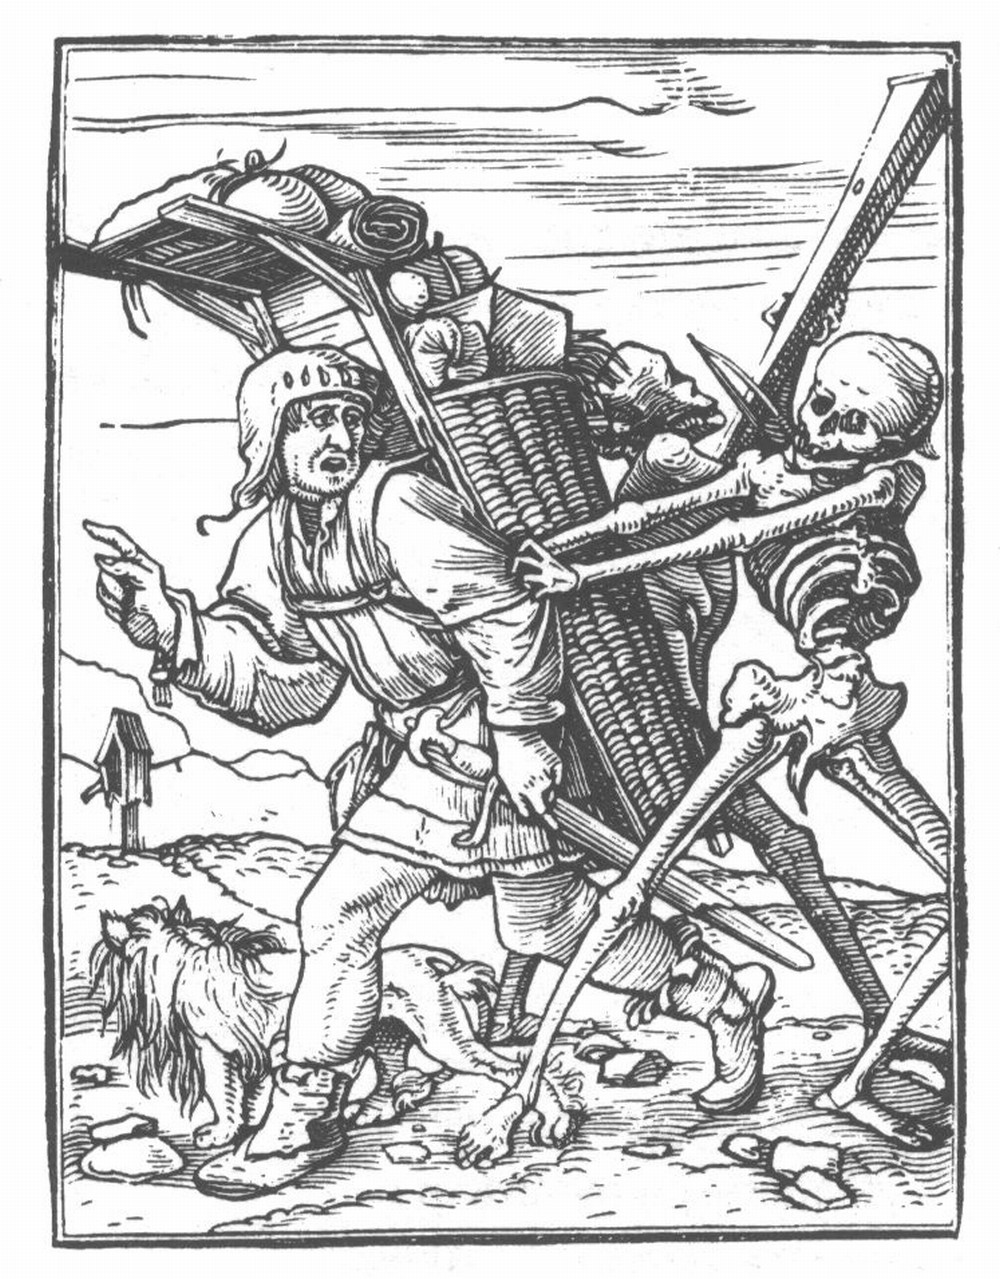
\includegraphics[scale=0.3]{imgs/exemplo}
		\end{lstlisting}
	O valor \verb|scale=0.3| é uma opção para definir que a imagem deve ter 30\% do seu tamanho original;
	
	\item \textbf{comentários:} além dos comandos, existem também os comentários, representados pelo sinal porcentagem (\texttt{\%}). Eles dizem para o interpretador do código que ignore todo o texto após o sinal. Em alguns casos (como quebras de linhas após abertura de colchetes), utiliza-se o sinal \texttt{\%} para que não haja espaços horizontais desnecessários.
\end{alineas}



\section{Comandos de Texto}

O \LaTeX\ oferece uma rica coleção de comandos dedicados à \textbf{formatação e estilização do texto}. Esses comandos permitem controlar a aparência do texto, como o estilo da fonte, o tamanho e a ênfase.
Aqui estão alguns dos comandos de texto mais frequentemente utilizados:

\begin{alineas}
	\item \textbf{ênfase e estilo da fonte:}
	\begin{alineas}
		\item \verb|\textbf{texto}|: produz texto em \textbf{negrito};
		\item \verb|\textit{texto}|: produz texto em \textit{itálico};
		\item \verb|\texttt{texto}|: produz texto em \texttt{monoespaçado} (fonte de máquina de escrever), útil para código ou nomes de arquivos;
		\item \verb|\textsf{texto}|: produz texto em \textsf{sans-serif} (sem serifa);
		\item \verb|\underline{texto}|: sublinha o \underline{texto};
		\item \verb|\emph{texto}|: aplica \emph{ênfase} ao texto. A forma como a ênfase é aplicada (itálico, negrito, etc.) pode depender do contexto e da classe do documento;
		\item \verb|\textsc{texto}|: gera texto em \textsc{SmallCaps}. Comum em nomes de algoritmos.
	\end{alineas}
	
	\item \textbf{tamanho da fonte:} o \LaTeX\  possui uma série de comandos para alterar o tamanho da fonte de forma relativa ao tamanho base do documento. É importante notar que estes comandos não aceitam argumentos e afetam todo o texto subsequente até que outro comando de tamanho seja utilizado, ou até o fim de um grupo delimitado por chaves:
	\begin{alineas}
		\item \verb|\tiny|: {\tiny texto muito pequeno;}
		\item \verb|\scriptsize|: {\scriptsize texto bem pequeno;}
		\item \verb|\footnotesize|: {\footnotesize texto pequeno;}
		\item \verb|\small|: {\small texto um pouco menor que o normal;}
		\item \verb|\normalsize|: {\normalsize tamanho de texto padrão (geralmente o padrão);}
		\item \verb|\large|: {\large texto grande;}
		\item \verb|\Large|: {\Large texto maior;}
		\item \verb|\LARGE|: {\LARGE texto ainda maior;}
		\item \verb|\huge|: {\huge texto enorme;}
		\item \verb|\Huge|: {\Huge texto realmente enorme.}
	\end{alineas}
	Para esse template, o comando mais importante é o \verb|\small|, que gera texto em 11pt, utilizado para notas, indicar a fonte de figuras e etc;
	
	\item \textbf{quebras de linha e espaçamento:}
	\begin{alineas}
		\item \verb|\\|: força uma quebra de linha;
		\item \verb|\newline|: também força uma quebra de linha, mas é mais robusto em alguns contextos;
		\item \verb|\linebreak|: sugere um ponto de quebra de linha, mas permite ao LaTeX ignorá-lo se não for ideal;
		\item \verb|\hspace{comprimento}|: insere um espaço horizontal com o comprimento especificado (ex: \verb|\hspace{1cm}|);
		\item \verb|\vspace{comprimento}|: insere um espaço vertical com o comprimento especificado (ex: \verb|\vspace{0.5cm}|).´
	\end{alineas}
	
	\item \textbf{listas e tabulações simples (para texto corrido):} embora existam ambientes específicos para listas (\texttt{itemize}, \texttt{enumerate}) e tabelas (\texttt{tabular}), para alinhamentos simples em texto corrido, podem ser usados:
	\begin{alineas}
		\item \verb|\quad| e \verb|\qquad|: inserem espaços horizontais fixos maiores.
		\item \verb|\tabto{posição}|: para alinhar texto em uma posição específica, embora seja mais complexo e menos comum para iniciantes.
	\end{alineas}
\end{alineas}

O domínio desses comandos de texto permite um controle preciso sobre a apresentação visual do seu documento, garantindo que a mensagem seja transmitida com a clareza e o impacto desejados.





\section{Figuras} \label{sec:latexFiguras}

\begin{figure}[htb!]
	\centering
	\caption{Uma Figura de Exemplo}\label{fig:exemplo} %legenda e referência
	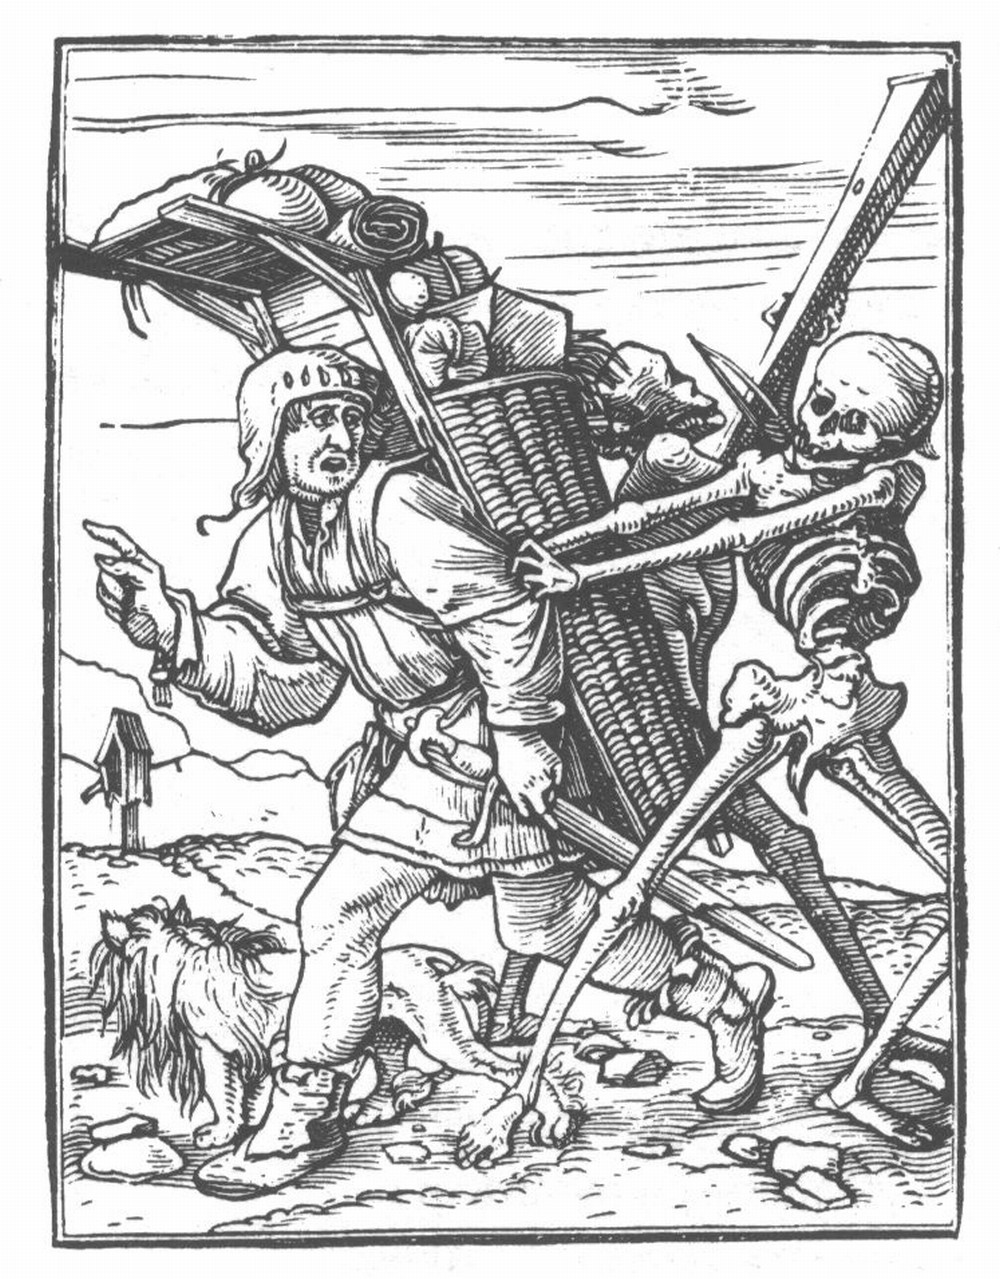
\includegraphics[scale=0.3]{imgs/exemplo}
	
	\fonte{fonte da figura (domínio público)} %Fonte da imagem
\end{figure}

A inclusão de \textbf{figuras} é um aspecto fundamental em muitos documentos, especialmente em trabalhos acadêmicos, relatórios técnicos e apresentações. O LaTeX, em conjunto com o pacote \texttt{graphicx}, oferece um controle robusto sobre a inserção, posicionamento e legendagem de imagens:

\begin{alineas}
	\item \textbf{o ambiente} \texttt{figure}\textbf{:} figuras no LaTeX são geralmente inseridas dentro do ambiente \texttt{figure}. Este é um ambiente "flutuante", o que significa que o LaTeX pode mover a figura para uma posição ideal na página para evitar quebras de página embaraçosas e garantir uma boa legibilidade. Em um comando:
	\begin{lstlisting}[language={[LaTeX]TeX}]
\begin{figure}[posicionamento]
	% Conteúdo da figura aqui
\end{figure}
	\end{lstlisting}
	As opções de posicionamento entre colchetes (\texttt{[]}) sugerem ao LaTeX onde tentar posicionar a figura:
	\begin{alineas}
		\item \texttt{h} (here): tenta colocar a figura exatamente onde ela aparece no código;
		\item \texttt{t} (top): coloca a figura no topo da página;
		\item \texttt{b} (bottom): coloca a figura na parte inferior da página;
		\item \texttt{p} (page): coloca a figura em uma página separada dedicada a figuras e tabelas;
		\item \texttt{H} (here, force): força a figura a ficar exatamente onde ela é colocada no código (requer o pacote `float`). Use com cautela.
	\end{alineas}
	
	\item \textbf{o comando} \verb|\includegraphics{}|\textbf{:} este é o comando principal para inserir arquivos de imagem. Ele deve ser usado dentro do ambiente \texttt{figure}.
	\begin{lstlisting}[language={[LaTeX]TeX}]
\includegraphics[opcoes]{nome_do_arquivo}
	\end{lstlisting}
	As opções são especificadas entre colchetes (\texttt{[]}) e permitem controlar o tamanho e a rotação da imagem:
	\begin{alineas}
		\item \texttt{width=largura}: define a largura da imagem (ex: \texttt{width=0.8}\verb|\linewidth| para 80\% da largura da linha);
		\item \texttt{height=altura}: define a altura da imagem;
		\item \texttt{scale=fator}: redimensiona a imagem por um fator (ex: \texttt{scale=0.5} para metade do tamanho original);
		\item \texttt{angle=graus}: rotaciona a imagem pelos graus especificados.
	\end{alineas}
	Os formatos de imagem suportados dependem do compilador LaTeX que você está usando (e.g., PDFLaTeX suporta PDF, PNG, JPG; LaTeX tradicional suporta EPS). Para gráficos e diagramas, formatos vetoriais são preferidos, como PDF ou EPS.
	
	\item \textbf{legendas e rótulos:}
	\begin{alineas}
		\item \verb|\caption{Texto da Legenda}|: adiciona uma legenda à figura. É fundamental para descrever o conteúdo da imagem e garantir que ela seja incluída na lista de figuras;
		\item \verb|\label{chave_referencia}|: cria um rótulo único para a figura. Isso permite referenciá-la em qualquer parte do texto usando \verb|\ref{chave_referencia}| (que gerará o número da figura) ou \verb|\autoref{chave_referencia}| (que gerará "Figura X"). Por exemplo, podemos referir à imagem de exemplo como \autoref{fig:exemplo} e o texto resultante, em PDF, será um link para a figura em questão.
	\end{alineas}
	
	\item \textbf{centralizando figuras:} é comum centralizar figuras na página para uma melhor apresentação. Isso pode ser feito usando o comando \verb|\centering| dentro do ambiente \texttt{figure}:
	\begin{lstlisting}[language={[LaTeX]TeX}]
\begin{figure}[!htb]
	\centering
	\caption{Uma Figura de Exemplo}\label{fig:exemplo} 
	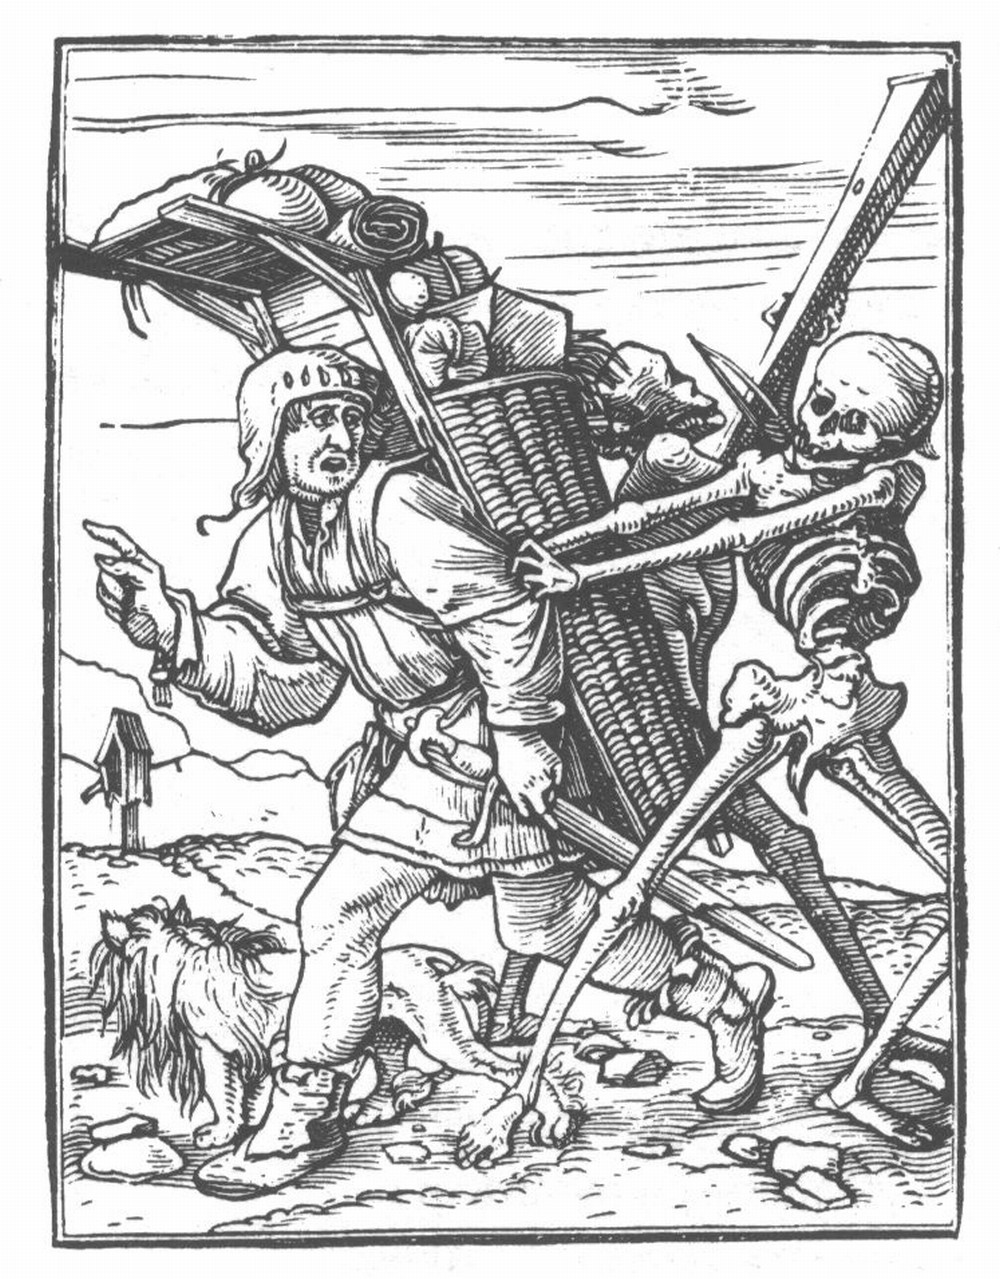
\includegraphics[scale=0.3]{imgs/exemplo}
	
	\fonte{fonte da figura (domínio público)} %Fonte da imagem
\end{figure}
	\end{lstlisting}
\end{alineas}

A correta utilização desses comandos e ambientes para figuras garante que suas ilustrações sejam incorporadas de forma profissional e acessível, complementando o conteúdo textual do seu documento.





\section{Ambientes Tabulares}

\begin{table}[h!]
	\centering
	\caption{Exemplo de Tabela Flutuante com Legenda}\label{tab:exemplo}
	\begin{tabular}{l c r}
		\hline
		\linhadir{Cabeçalho 1} & \linhadir{Cabeçalho 2} & Cabeçalho 3 \\
		\hline
		Item 1 & Valor A & Nota X \\
		Item 2 & Valor B & Nota Y \\
		\hline
	\end{tabular}
	
	\vspace{.3cm}
	\fonte{original}
\end{table}

Tabelas são elementos cruciais para apresentar dados de forma organizada e legível em documentos científicos e acadêmicos. No \LaTeX, a criação de elementos tabulares é feita principalmente através do ambiente \texttt{tabular}, que oferece um controle preciso sobre a formatação e o alinhamento do conteúdo.

A estrutura fundamental de uma tabela em \LaTeX\  envolve o ambiente \texttt{tabular} e o uso de especificadores para definir o alinhamento das colunas e as linhas divisórias. Veja um exemplo simples:

\begin{lstlisting}[language={[LaTeX]TeX}]
\begin{tabular}{l c r}
  \hline
  \linhadir{Cabeçalho 1}& \linhadir{Cabeçalho 2}& Cabeçalho 3\\
  \hline
  Item 1& Valor A& Nota X\\
  Item 2& Valor B& Nota Y\\
  \hline
\end{tabular}
\end{lstlisting}
Nesse exemplo:

\begin{alineas}
	\item \texttt{\textbackslash begin\{tabular\}\{...\}} e \texttt{\textbackslash end\{tabular\}} delimitam o ambiente da tabela.
	\item os caracteres dentro das chaves \texttt{\{...\}} definem a formatação das colunas:
	\begin{alineas}
		\item \texttt{l} (left): alinha o conteúdo à esquerda;
		\item \texttt{c} (center): centraliza o conteúdo;
		\item \texttt{r} (right): alinha o conteúdo à direita;
		\item \texttt{|}: adiciona uma linha vertical entre as colunas.
	\end{alineas}
	\item \texttt{\&} é usado para separar o conteúdo de cada célula em uma linha;
	\item \texttt{\textbackslash\textbackslash} indica o fim de uma linha e o início da próxima;
	\item \texttt{\textbackslash hline} insere uma linha horizontal que abrange toda a largura da tabela.
\end{alineas}

\vspace{\baselineskip}

Para que sua tabela seja tratada como um ``float'' (flutuante), permitindo que o \LaTeX\  decida a melhor posição para ela no documento, e para que você possa adicionar uma legenda e referenciá-la, você deve encapsular o ambiente \texttt{tabular} dentro de um ambiente \texttt{table} ou \texttt{quadro}:

\begin{lstlisting}[language={[LaTeX]TeX}]
\begin{table}[h!]
	\centering
	\caption{Exemplo de Tabela Flutuante com Legenda}
	\label{tab:minhatabela}
	\begin{tabular}{l c r}
		\hline
		\linhadir{Cabeçalho 1}& \linhadir{Cabeçalho 2}& Cabeçalho 3\\
		\hline
		Item 1 & Valor A & Nota X \\
		Item 2 & Valor B & Nota Y \\
		\hline
	\end{tabular}

	\vspace{.3cm}
	\fonte{original}
\end{table}
\end{lstlisting}

Os comandos usados e suas explicacões são:
\begin{alineas}
	\item \texttt{\textbackslash begin\{table\}[h!]} e \texttt{\textbackslash end\{table\}}: delimitam o ambiente flutuante da tabela. As opções entre colchetes, como \texttt{[h!]}, sugerem ao \LaTeX\  a preferência de posicionamento (\texttt{h} para ``here'' - aqui, \texttt{!} para ``definitivamente aqui se possível''). Outras opções incluem \texttt{t} (top - topo da página), \texttt{b} (bottom - base da página) e \texttt{p} (page of floats - página dedicada a flutuantes);
	\item \texttt{\textbackslash centering}: centraliza a tabela na página;
	\item \texttt{\textbackslash caption\{...\}}: adiciona uma legenda à tabela;
	\item \texttt{\textbackslash label\{...\}}: permite criar uma referência cruzada para a tabela usando\\ \texttt{\textbackslash ref\{tab:minhatabela\}} no texto, que será automaticamente atualizada com o número da tabela ou quadro, como \autoref{tab:exemplo}.
\end{alineas}

\subsection{Formatação Avançada}

O \LaTeX\  oferece diversas opções para customizar suas tabelas, incluindo:

\begin{alineas}
	\item \textbf{linhas horizontais parciais:} use \texttt{\textbackslash cline\{i-j\}} para desenhar uma linha horizontal apenas das colunas \texttt{i} a \texttt{j};
	\item \textbf{células mescladas:} o pacote \texttt{multirow} permite mesclar células verticalmente\\ (\texttt{\textbackslash multirow\{num\_linhas\}\{largura\}\{conteúdo\}}) e o \texttt{multicolumn}\\ horizontalmente (\texttt{\textbackslash multicolumn\{num\_colunas\}\{alinhamento\}\{conteúdo\}});
	\item \textbf{espaçamento:} é possível ajustar o espaçamento entre linhas e colunas, além de usar pacotes como \texttt{booktabs} para criar tabelas com uma aparência mais profissional, focando em linhas mais finas e espaçamento aprimorado para melhorar a legibilidade.
\end{alineas}

Aprender a manipular tabelas no \LaTeX\  pode parecer complexo no início, mas o controle que ele oferece resulta em documentos com um visual extremamente polido e profissional, mantendo a consistência em todo o seu trabalho.


\section{Elementos Matemáticos}

Lidar com equações e símbolos complexos é uma das maiores vantagens do \LaTeX. Para inserir elementos matemáticos, você precisa estar em um \textbf{ambiente matemático}. Existem dois tipos principais de ambientes matemáticos:

\begin{alineas}
	\item \textbf{matemática em linha (inline math):} usada para equações curtas e símbolos que aparecem dentro do texto. Para entrar neste modo, você pode usar os delimitadores \verb|$$| ou \verb|\( ... \)|.\\
	Por exemplo: a frase ``a equação $E=mc^2$ é famosa. Ou, alternativamente, a equação \(E=mc^2\) é famosa'' pode ser escrita com:
	\begin{lstlisting}[language={[LaTeX]TeX}]
A equação $E=mc^2$ é famosa. Ou, alternativamente, a
equação \(E=mc^2\) é famosa. 
	\end{lstlisting}
	
	\item \textbf{matemática em exibição (display math):} usada para equações maiores que precisam de uma linha própria e que muitas vezes são numeradas. Para entrar neste modo, você pode usar os delimitadores \verb|$$| ou \verb|\[ ... \]|. A maneira mais comum e recomendada é usar o ambiente \texttt{equation} ou \texttt{align} (do pacote \texttt{amsmath}).\\
	Por Exemplo:
	\begin{lstlisting}[language={[LaTeX]TeX}]
$$
	\int_a^b f(x) \, dx = F(b) - F(a)
$$
	\end{lstlisting}
	Ou, preferencialmente:
	\begin{lstlisting}[language={[LaTeX]TeX}]
\begin{equation}
	\int_a^b f(x) \, dx = F(b) - F(a)
\end{equation}
	\end{lstlisting}
	O ambiente \texttt{equation} numera automaticamente a equação. Se você não quiser numerar, use \texttt{equation*}.
\end{alineas}



\subsection{Símbolos e Estruturas Comuns}

\LaTeX\ oferece uma vasta gama de símbolos e estruturas matemáticas. Aqui estão alguns dos mais utilizados:

\begin{alineas}
	\item \textbf{expoentes e subscritos:} use \verb|^| para expoentes e \verb|_| para subscritos. Se houver mais de um caractere, agrupe-os com chaves \verb|{}|:\\
	\textbf{Exemplo:} $x^2$, $a_{ij}$, $e^{i\pi}$.
	\begin{lstlisting}[language={[LaTeX]TeX}]
	$x^2$, $a_{ij}$, $e^{i\pi}$
	\end{lstlisting}
	
	
	\item \textbf{frações:} use \verb|\frac{numerador}{denominador}|:\\
	\textbf{Exemplo:} $\frac{1}{2}$, $\frac{x+y}{x-y}$.
	\begin{lstlisting}[language={[LaTeX]TeX}]
	$\frac{1}{2}$, $\frac{x+y}{x-y}$
	\end{lstlisting}
	
	\item \textbf{raízes:} use \verb|\sqrt{argumento}| para raiz quadrada e \verb|\sqrt[n]{argumento}| para a raiz n-ésima:\\
	\textbf{Exemplo:} $\sqrt{2}$, $\sqrt[3]{x^2+y^2}$.
	\begin{lstlisting}[language={[LaTeX]TeX}]
	$\sqrt{2}$, $\sqrt[3]{x^2+y^2}$
	\end{lstlisting}
	
	\item \textbf{somas e integrais:} use \verb|\sum| para somatórios e \verb|\int| para integrais. Os limites inferior e superior são adicionados com \verb|_| e \verb|^|, respectivamente:\\
	\textbf{Exemplo:} $\sum_{i=1}^n i^2$, $\int_a^b x^2 \, dx$.
	\begin{lstlisting}[language={[LaTeX]TeX}]
	$\sum_{i=1}^n i^2$, $\int_a^b x^2 \, dx$
	\end{lstlisting}
	
	\item \textbf{parênteses, colchetes e chaves ajustáveis:} para que os delimitadores se ajustem ao tamanho do conteúdo interno, use \verb|\left(| e \verb|\right)|, \verb|\left[| e \verb|\right]|, ou \verb|\left\{| e \verb|\right\}|:\\
	\textbf{Exemplo:} $\left(\frac{1}{2}\right)$, $\left[\sum_{i=1}^n x_i\right]$.
	\begin{lstlisting}[language={[LaTeX]TeX}]
	$\left(\frac{1}{2}\right)$,
		$\left[\sum_{i=1}^n x_i\right]$
	\end{lstlisting}
	
	\item \textbf{letras gregas:} basta digitar o nome da letra com uma barra invertida antes (a primeira letra maiúscula para a versão maiúscula):\\
	\textbf{Exemplo:} $\alpha$, $\beta$, $\Gamma$, $\Delta$.
	\begin{lstlisting}[language={[LaTeX]TeX}]
	$\alpha$, $\beta$, $\Gamma$, $\Delta$
	\end{lstlisting}
	
	\item \textbf{operadores matemáticos:} existem comandos para operadores como \verb|\sin|, \verb|\cos|, \verb|\log|, \verb|\lim|, etc:\\
	\textbf{Exemplo:} $\sin(x)$, $\log_2(x)$,$\lim_{x \to 0}\frac{\sin x}{x}$.
	\begin{lstlisting}[language={[LaTeX]TeX}]
	$\sin(x)$, $\log_2(x)$, 
		$\lim_{x \to 0}\frac{\sin x}{x}$
	\end{lstlisting}
	
\end{alineas}

\subsection{Pacote \texttt{amsmath}}

Para composições matemáticas mais avançadas e eficientes, é altamente recomendável incluir o pacote \texttt{amsmath} no preâmbulo do seu documento (\verb|\usepackage{amsmath}|). Ele oferece ambientes como \texttt{align} para alinhar múltiplas equações, \texttt{gather} para agrupar equações e muitos outros comandos úteis.

\subsection{Exemplo de Equação}
Abaixo, temos um exemplo de uma equação, utilizando o ambiente \texttt{equation}, que pode ser referenciada como \autoref{eq:exemplo}:


\begin{equation}
	\label{eq:exemplo}
	f(x) = \sum_{n=1}^{\infty} f^{(n)}(x)~~\frac{(x-a)^n}{n!}
\end{equation}


\section{Usando Referências}\label{sec:Refs}

Para gerenciar referências bibliográficas de forma eficiente no \LaTeX, pode-se utilizar o BibTeX. Ele permite que você mantenha sua bibliografia em um arquivo separado, tornando o processo de citação e a geração da lista de referências muito mais organizado e automatizado.

\subsection{Arquivo \texttt{.bib}}

Primeiro, é necessário um arquivo com a extensão \texttt{.bib} (por exemplo, \texttt{refbib.bib}). Neste arquivo, devem ser definidas todas as entradas bibliográficas usando um formato específico do BibTeX. É comum publicações online disponibilizarem entradas BibTeX prontas. O exemplo de uma entrada é:
\begin{lstlisting}[language={[LaTeX]TeX}]
@Manual{Weber2003,
	Title          = {Estilo bibtex compatível com a `norma' 6023/2000 da {ABNT}},
	Author         = {Gerald Weber},
	Organization   = {Grupo abnTeX},
	URL            = {http://abntex.codigolivre.org.br},
	year           = 2003
}
\end{lstlisting}
Existem diversos tipos de entrada (como \texttt{@book}, \texttt{@inproceedings}, \texttt{@misc}) e campos obrigatórios/opcionais para cada um.

\subsection{Citando no Texto}
Para citar uma referência em seu texto, use o comando \verb|\cite{chave}|, onde chave é o identificador único que você definiu no seu arquivo \texttt{.bib}.\\
Por exemplo, ``Exemplo da citação com cite: \cite{Weber2003}.'' tem código:
\begin{lstlisting}[language={[LaTeX]TeX}]
Exemplo da citação com cite: \cite{Weber2003}.
\end{lstlisting}

\subsection{Gerando Lista de Referências}
A lista de referências será gerada automaticamente no local onde você inserir o comando \verb|\bibliography{nomedoarquivo}|. Com \texttt{nomedoarquivo} sendo o nome do seu arquivo \texttt{.bib} (sem a extensão). As referências podem assumir diferentes estilos que podem ser alterados com o comando \verb|\bibliographystyle{estilo}|, com o estilo \texttt{plain}, por exemplo, gerando referências simples e enumeradas.
\chapter{\MakeUppercase{Utilizando a Classe no Formato da UFLA}}\label{sec:template}

Agora que já temos o conhecimento básico sobre como a linguagem \LaTeX\ funciona, podemos nos aprofundar nos detalhes de como utilizar esse template (e, especialmente, a classe \texttt{templufla}) para gerar documentos padronizados de alta qualidade.

\section{Sobre as Seções (seção secundária)}\label{sec2:secoes}
\subsection{Sobre as Seções (seção terciária com texto extra comicamente grande para testar como será a quebra de linha do título)}\label{sec3:teste}
\subsubsection{Sobre as Seções (seção quaternária)}\label{sec4:teste}
\subsubsubsection{Sobre as Seções (seção quinária)}\label{sec5:teste}

Um dos fatores fundamentais no desenvolvimento de um trabalho acadêmico é sua organização. Na normalização da UFLA e da ABNT, os trabalhos podem ter formato de livro, como esse template, mas devem ser divididos em seções, não em capítulos e todo o texto pode ser dividido até a seção quinária.

No template, dispõem-se comandos para realizar tal divisão automaticamente, mas com uma importante observação: a seção primária utiliza o comando \verb|\chapter|. Isso foi feito para simplificar a migração de versões mais antigas e provavelmente será alterado no futuro. Abaixo estão listados os comandos de seccionamento disponíveis: 

\begin{alineas}
	\item \verb|\chapter|:  cria uma seção primária, que pode ser referenciada como \autoref{sec:template};
	\item \verb|\section|:  cria uma seção secundária, que pode ser referenciada como \autoref{sec2:secoes};
	\item \verb|\subsection|:  cria uma seção terciária, que pode ser referenciada como \autoref{sec3:teste};
	\item \verb|\subsubsection|:  cria uma seção quaternária, que pode ser referenciada como \autoref{sec4:teste};
	\item \verb|\subsubsubsection|:  cria uma seção quinária, que pode ser referenciada como \autoref{sec5:teste}.
\end{alineas}


\section{Alíneas e Subalíneas}
Segundo a normalização \cite{UFLA:2025}, ``as alíneas são usadas quando se deseja enumerar diversos assuntos de uma seção sem título próprio. Quando necessário, a alínea pode ser dividida em subalíneas.''

Nesse template, para listar elementos com alíneas, deve-se usar o ambiente \textbf{\texttt{alineas}}, que pode ser aninhado para criar subalíneas: 
\begin{lstlisting}[language={[LaTeX]TeX}]
	\begin{alineas}% [labelsep=0ex]
		\item item um;
		\item item dois:
		\begin{alineas} % subalíneas
			\item subitem 1;
			\item subitem 2.
		\end{alineas}
	\end{alineas}
\end{lstlisting}
Caso tenham letras duplicadas e queira mais espaço entre o indicador e o texto, basta adicionar a opção \texttt{[labelsep=0ex]} ao ambiente.

\vspace{18pt}
Abaixo é mostrado exemplo em texto retirado, na maior parte, do manual:
\begin{alineas}% adicione [labelsep=0ex] caso tenha letras duplicadas e queira mais espaço
	\item as alíneas são formadas pelos diversos assuntos que não possuem título próprio, dentro de uma mesma seção;
	\item o texto que antecede as alíneas termina em dois pontos;
	\item as alíneas devem ser indicadas alfabeticamente, em letra minúscula, seguida de parêntese. Utilizam-se letras dobradas, quando esgotadas as letras do alfabeto;
	\item as letras indicativas das alíneas devem apresentar recuo em relação à margem esquerda;
	\item o texto da alínea deve começar por letra minúscula e terminar em ponto e vírgula, exceto a última alínea que termina em ponto final;
	\item o texto da alínea deve terminar em dois pontos, se houver subalínea;
	\item a segunda e as seguintes linhas do texto da alínea começam sob a primeira letra do texto da própria alínea;
	\item sobre as subalíneas:
	\begin{alineas}
		\item as subalíneas devem começar por travessão seguido de espaço;
		\item as subalíneas devem apresentar recuo em relação à alínea;
		\item o texto da subalínea deve começar por letra minúscula e terminar em ponto e vírgula. A última subalínea deve terminar em ponto final, se não houver alínea subsequente;
		\item a segunda e as seguintes linhas do texto da subalínea começam sob a primeira letra do texto da própria subalínea;
		\item o recuo das margens também deve ser obedecido.
	\end{alineas}
\end{alineas}


\section{Figuras, Ilustrações e etc}

Utilizar figuras, ilustrações e elementos ``float'' no template é semelhante ao que foi explicado na \autoref{sec:latexFiguras}.
\begin{figure}[h]
	\centering
	\caption{Leão do site CTAN estudando \TeX}
	\label{fig:leaoCTAN}
	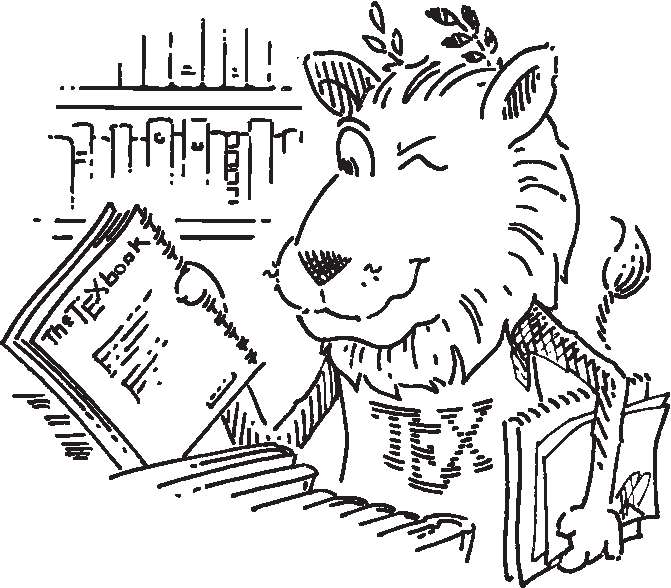
\includegraphics[width=0.6\textwidth]{imgs/ctanlion}
	\fonte{Duane Bibby, diponibilizado em \url{www.ctan.org/lion}}
\end{figure}


 Só é importante se atentar para dois detalhes: os títulos das figuras, que devem vir antes do \texttt{inludegraphics}, e a fonte, que deve ser posicionada após o \texttt{inludegraphics} e pode utilizar o comando pré definido \texttt{fonte}. Exemplo do código para a \autoref{fig:leaoCTAN}:
\begin{lstlisting}[language={[LaTeX]Tex}]
\begin{figure}
	\centering
	% \caption antes da figura
	\caption{Leão do site CTAN estudando \TeX} 
	\label{fig:leaoCTAN}
	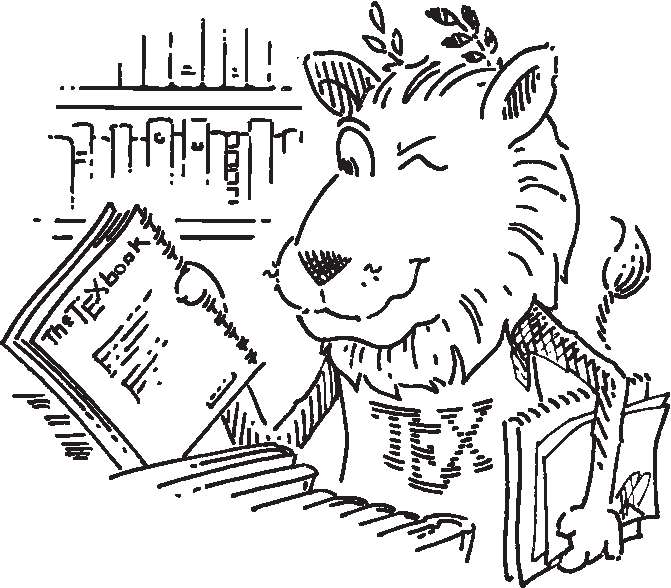
\includegraphics[width=0.6\textwidth]{imgs/ctanlion}
	\fonte{Duane Bibby, diponibilizador por \url{www.ctan.org}}
\end{figure}
\end{lstlisting}



\section{Quadros e Tabelas}\label{sec:tabelasUFLA}

A normalização da UFLA reconhece dois principais tipos de elementos tabulares, tabelas e quadros, com conteúdos e formatos específicos. 

\begin{table}[h]
	\centering
	\caption{Exemplo de Tabela} 
	\label{tab:exemplo2}
	\begin{tabular}{c c c c }
		\hline
		\linhadir{\bf Pessoa} & \linhadir{\bf Livros} & \linhadir{\bf Artigos} & \bf Palestras \\
		\hline
		$p_1$ & 1 & 3 & 4 \\
		$p_2$ & 1 & 3 & 3 \\
		$p_3$ & 1 & 3 & 4 \\
		$p_4$ & 3 & 5 & 2 \\
		\hline 
	\end{tabular}
	\vspace{0.3cm}
	\fonte{original} %Fonte do tabela
\end{table}

Tabelas envolvem principalmente números, utiliza-se linhas horizontais somente no topo, final e cabeçalhos, além disso utiliza-se linhas verticais somente nos cabeçalhos\footnote{Por isso a \autoref{tab:exemplo} não segue o padrão correto.}. Para reduzir o tamanho do código dos cabeçalhos, a classe \texttt{templufla} define do comando \texttt{linhadir}, que adiciona uma linha vertical à direita da célula. Abaixo mostra-se um exemplo do código para a \autoref{tab:exemplo2}:
\begin{lstlisting}[language={[LaTeX]Tex}]
\begin{table}[h]
	\centering
	\caption{Exemplo de Tabela} 
	\label{tab:exemplo2}
	\begin{tabular}{c c c c }
		\hline
		\linhadir{Pessoa}& \linhadir{Livros}& \linhadir{Artigos}& Palestras\\
		\hline
		$p_1$& 1& 3& 4\\
		$p_2$& 1& 3& 3\\
		$p_3$& 1& 3& 4\\
		$p_4$& 3& 5& 2\\
		\hline 
	\end{tabular}
	\vspace{0.3cm}
	\fonte{original} %Fonte do tabela
\end{table}
\end{lstlisting}


Quadros se diferem das tabelas por conterem principalmente dados textuais e suas células serem completamente fechadas. O \autoref{quad:exemplo} é um exemplo de quadro.

\begin{quadro}[h]
\centering
\caption{Opiniões sobre esse template}\label{quad:exemplo}
  \begin{tabular}{|l|p{9cm}|}
    \hline 
    \rowcolor[gray]{.9}
    \bf Nome& \bf Opinião\\
    \hline
    Jão& Desculpe, não posso comentar sobre isso.\\
    \hline
    Joana& Literalmente uma revolução do cinema nacional!\\
    \hline
    Jacquin& Esse autor é a vergonha da profisson!\\
    \hline
    Meu cachorro& Au! Au! Au! $\sim$Sons de papel sendo rasgado.\\
    \hline
    Overleaf& ASSINE, ASSINE O PREMIUM.\\
    \hline
    \end{tabular}
    
    \vspace{0.3cm}
	\fonte{original}
\end{quadro}


\section{Padrão das Referências}

Desde que o padrão descrito na \autoref{sec:Refs} seja seguido e partes importantes do template sejam mantidas, as referências não devem ser um problema. O template já vem configurado para o formato padrão da ABNT, desde que os arquivos \texttt{abntex.*}, o preâmbulo e a chamada dos comandos \texttt{bibliographystyle}, \texttt{citeoption}, \texttt{refencias} e \texttt{bibliography}, próximos ao final do arquivo principal, sejam mantidos.

É comum referências serem um problema e, apesar do \LaTeX\ ajudar muito nisso, o processo ainda pode ser complicado. O pacote \texttt{abntex2} está desatualizado, as correções precisaram ser \emph{hard-coded} e o arquivo principal reflete isso.

\textbf{Então, se você quer que as citações e referências sejam tão simples quanto adicionar um \texttt{bibtex} e usar o comando \texttt{cite}, EU TE SUPLICO, não altere o preâmbulo nem os comandos relacionados às referências no \texttt{tempulfa\_main.tex}.}

Referências sortidas para contribuir para a lista ao final (ignore): \cite{Eco1996,Booth2000,BIB2010,Hexsel2004,Franca2001,Gil2002,Porto2002,Silva2005,UFLA:2015,Moura1998,NBR6023:2002,LeGuin:1987}


\chapter{LISTAS, GLOSSÁRIO E ÍNDICE}\label{sec:listasEGlossario}

O template também inclui a criação dos elementos pré-textuais lista de abreviações (ou, como está no manual, abreviaturas), siglas e símbolos. Além disso, também inclui a criação do glossário e índice.

Todos esses novos elementos, exceto o índice, utilizam o mesmo pacote, \texttt{glossaries}, então, têm comportamento semelhante. Cada ítem deve ser adicionado aos glossários no preâmbulo e, após adicionados, podem ser referenciados no documento com o comando \texttt{gls}. Por exemplo:
	
\begin{figure}[!htb]
	\centering
	\caption{Inserindo ítem no \gls{glo:glossario} e o referindo no texto} %legenda
	\label{fig:exemploglossario1} %rotulo para refencia
	\begin{lstlisting}[language=tex]
\newglossaryentry{glo:glossario}{
	name={glossário}, 
	description={
		Relação de palavras ou expressões técnicas 
		de uso restrito ou de sentido obscuro, 
		utilizadas no texto, acompanhadas das 
		respectivas definições}
	}
		
%\makeglossaries % não é necessario nesse template pois já é chamado na classe
\begin{document}
...
\caption{Inserindo ítem no gls(glo:glossario) e o referindo no texto}
	\end{lstlisting}
	
	\fonte{original}
\end{figure}

O comando \textit{\textbf{gls}} escreve o nome do ítem quando é usado. Para que outro valor seja escrito, ou até para que nada seja escrtio, pode-se utilizar o comando \texttt{glslink}:
\begin{lstlisting}[language=tex]
	\glslink{<rótulo>}{<texto alternativo>}
\end{lstlisting}

É recomendável separar as adições aos glossários em arquivos para melhor organização e reduzir o tamanho do preâmbulo. Nesse template, cada glossário tem seu próprio arquivo, adicionado ao projeto via comandos \texttt{loadglsentries}, e os arquivos têm sua própria pasta. Essa organização pode ser alterada, desde que a mudança seja refletida no preâmbulo.

\newpage
Abaixo listamos o formato para a adição de ítens em cada glossário:

\begin{alineas}
	\item \textbf{abreviaturas}: Adicionar uma abreviatura é simples e a sintaxe é relativamente fixa.\\ Um exemplo para a abreviatura de \gls{jan}:
		\begin{lstlisting}[language=tex]
\newabbreviation{jan} % rótulo
{jan.}% forma abreviada
{Janeiro} % forma completa
...
... Um exemplo para a abreviatura de \gls{jan}:
		\end{lstlisting}
	
	\item \textbf{siglas}: Adicionar siglas é igualmente simples.\\ 
	Um exemplo para a sigla \gls{abnt}:
	\begin{lstlisting}[language=tex]
\newacronym{abnt} % rótulo
{ABNT} % sigla
{Associação Brasileira de Normas Técnicas} % nome completo
...
... Um exemplo para a sigla \gls{abnt}:
	\end{lstlisting}
	
	\item \textbf{símbolos}: Adicionar símbolos é um pouco mais complicado, já que necessita de uma descrição. Como a lista é por ordem de uso, \gls{gama} deve aparecer antes de \gls{alfa}\\ 
	Um exemplo para o símbolo \gls{gama}:
	\begin{lstlisting}[language=tex]
\newglossaryentry{gama}{
	name={$\gamma$}, % o símbolo em questão
	description={Um número gama}, % descrição do símbolo
	type={symbols}} % indicador que é um símbolo
...
... Um exemplo para o símbolo \gls{gama}:
	\end{lstlisting}
	
	\item \textbf{glossário}: Adicionar termos no glossário é igual ao exemplo mostrado antes.\\
	Nesse caso, no entanto, adicionamos uma \emph{tag} \LaTeX\ antes do nome, então temos que adicionar o valor "\emph{sort}", para que a ordenação seja correta.
	Um exemplo para o termo \gls{llm}:
	\begin{lstlisting}[language=tex]
\newglossaryentry{llm}{
	name={\emph{large language model}}, % o nome do termo
	description={Grande model de 
		linguagem. Ex:DeepSeek-R1}, % descrição do termo
	sort={large language model}} % chave para ordenação
...
... Um exemplo para o termo \gls{llm}:
	\end{lstlisting}
	
	\item \textbf{índice}: Adicionar termos ao índice é o mais fácil de todos. Para adicionar um índice, basta utilizar o comando \emph{index}. Caso algum índice tiver um pai(ou mãe), basta adicionar o delimitador ``!''.\\
	Um exemplo para os termos conjunto\index{Conjunto}, conjunto aberto\index{Conjunto!aberto} e conjunto fechado\index{Conjunto!fechado}:
	\begin{lstlisting}[language=tex]
...Um exemplo para os termos conjunto\index{Conjunto},
conjunto aberto\index{Conjunto!aberto} e conjunto 
fechado\index{Conjunto!fechado}:
	\end{lstlisting}
	
\end{alineas}

Para mais informações sobre como usar esses pacotes, consulte as documentações oficiais do \texttt{glossaries}\footnote{https://ctan.org/pkg/glossaries?lang=en} e do \texttt{imakeidx}\footnote{https://ctan.org/pkg/imakeidx}.

\chapter{\MakeUppercase{Conclusão}}\label{sec:conclusao}

O objetivo deste documento foi apresentar o uso básico da classe \texttt{templufla} para a elaboração de trabalhos acadêmicos da UFLA utilizando \LaTeX. Após edição em \LaTeX, o usuário pode gerar arquivos PDF \cite{PDF2004} ou PostScript \cite{PostScript1999} com grande facilidade.



%==============================================================================
% Bibliografia

% Carrega o estilo para referências ABNT
\bibliographystyle{abntex2-alf}            

% Alterando informações do estilo de citação.
% Como estamos usando uma versão alterada, essas opções são necessárias.
% Et al. em itálico
\citeoption{abnt-etal-text=it}

% Até 3 autores antes do et al.
\citeoption{abnt-etal-cite=3}

% Colocar s.d. na falta de um ano de publicação
\citeoption{abnt-missing-year=sd}

% Altera o estilo de citação para (Autor, ano)
% A opção abnt-cite-style=AuthorYEAR está quebrada; essa é equivalente.
\citeoption{abnt-nbr10520=1988} 


% Comando necessário para corrigir o título das referências.
% Para o estilo ABNT, esse comando SEMPRE deve ser
% chamado antes do \bibliography
\referencias
% Adiciona as referência em bibtex 
\bibliography{refbib}

%==============================================================================
% Outros elementos pós-textuais

% Glossário
\glossario

% Anexos e apêndices
% Os anexos devem ser includios antes
% e utilizar \input ao invés de \include, para não criar uma nova página
% Anexos
\anexo{Lorem Ipsum}\label{anex:lorem1}

Lorem ipsum dolor sit amet, consectetur adipiscing elit. Vivamus semper, libero egestas pellentesque vulputate, velit felis commodo ante, vel bibendum velit turpis eu felis. Donec viverra quam nisi, vel tincidunt enim tristique interdum. Integer tincidunt a lectus vel porttitor. Nulla venenatis vitae enim ut semper. Nunc in sagittis massa, sit amet dapibus quam. Mauris cursus, ligula ac pretium imperdiet, lectus libero egestas mi, quis tristique leo urna nec erat. In vitae dui maximus, imperdiet massa euismod, auctor enim. Morbi urna odio, accumsan quis magna id, fringilla gravida purus. Aenean facilisis est nisi, nec porttitor purus ullamcorper ut. Proin ac risus congue, aliquet elit in, cursus est.

Vivamus lorem diam, molestie ut ultrices at, feugiat quis tortor. Mauris feugiat, augue at molestie malesuada, purus erat sagittis tellus, sit amet posuere lacus nisl non eros. Sed enim justo, sagittis id elementum quis, commodo ut nibh. Aenean mauris odio, efficitur vel purus sit amet, molestie pharetra arcu. Nunc vel eros sodales, aliquam diam eu, rutrum nisi. Morbi non scelerisque diam. Suspendisse sed dapibus mi, ut sagittis nunc. Praesent ornare, est in rutrum dapibus, tortor massa ornare dolor, at ullamcorper metus augue et ipsum. Sed ut nulla in dolor aliquet faucibus. Quisque rhoncus auctor tellus eu lobortis. Proin rhoncus nisi sit amet nibh tempor hendrerit.\footnote{Lorem ipsum dolor sit amet, consectetur adipiscing elit. Vivamus semper, libero egestas pellentesque vulputate, velit felis commodo ante, vel bibendum velit turpis eu felis. Donec viverra quam nisi, vel tincidunt enim tristique interdum. Integer tincidunt a lectus vel porttitor.}
\anexo{Lorem Ipsum pt. 2}\label{anex:lorem2}

Aliquam tempus vehicula risus sit amet consequat. Donec eu mattis lorem. Maecenas tincidunt a massa ut ultricies. Ut id lacus sapien. Suspendisse ac auctor lectus. Maecenas vehicula sagittis metus, eget luctus ipsum imperdiet at. Nullam eu vestibulum leo. Fusce mauris ligula, consequat ut felis a, ornare bibendum quam. Maecenas posuere sem sit amet volutpat interdum. Integer aliquet bibendum luctus. Nulla non viverra eros. Fusce egestas scelerisque augue ac tempor.


Aliquam tempus vehicula risus sit amet consequat. Donec eu mattis lorem. Maecenas tincidunt a massa ut ultricies. Ut id lacus sapien. Suspendisse ac auctor lectus. Maecenas vehicula sagittis metus, eget luctus ipsum imperdiet at. Nullam eu vestibulum leo. Fusce mauris ligula, consequat ut felis a, ornare bibendum quam. Maecenas posuere sem sit amet volutpat interdum. Integer aliquet bibendum luctus. Nulla non viverra eros. Fusce egestas scelerisque augue ac tempor.


Aliquam tempus vehicula risus sit amet consequat. Donec eu mattis lorem. Maecenas tincidunt a massa ut ultricies. Ut id lacus sapien. Suspendisse ac auctor lectus. Maecenas vehicula sagittis metus, eget luctus ipsum imperdiet at. Nullam eu vestibulum leo. Fusce mauris ligula, consequat ut felis a, ornare bibendum quam. Maecenas posuere sem sit amet volutpat interdum. Integer aliquet bibendum luctus. Nulla non viverra eros. Fusce egestas scelerisque augue ac tempor.

% Apendices
\apendice{O que são apêndices}
\label{cap:apendice}

Um apêndice é um suporte elucidativo e ilustrativo do texto principal. Sua função é agrupar elementos que são úteis à compreensão do texto e que, no entanto, podem ser apresentados à parte sem prejuízo à compreensão. É útil para a apresentação de modelagens, diagramas extensos, listagens de código-fonte de programas e demais elementos que o autor julgar necessário à complementação do tema abordado no texto principal.

% Índice
\indice


%==============================================================================
% Fim do documento
%==============================================================================
\end{document}
